\subsection{Apparato sperimentale}\label{subsec:apparato-sperimentale}
  L’apparato sperimentale è riportato in Fig.\ref{fig:apparato-strumentale}.
  Un prisma(5) di vetro \emph{crown} è posizionato all centro di una guida circolare graduata(4),
  montato ad un servomotore \emph{SM-S2309S}\footnote{http://descargas.cetronic.es/microservo.pdf}.
  Un laser(1) a luce rossa e due filtri polaroid(2, 3) sono
  allineati con il prisma. Un sensore di intensità luminosa(6) \emph{TEMT6000}\footnote{https://www.sparkfun.com/datasheets/Sensors/Imaging/TEMT6000.pdf},
  collegato ad un microcontrollore(7) \emph{Arduino Uno (ATmega328)}\footnote{http://store.arduino.cc/products/arduino-uno-rev3}
  \footnote{Da qui in avanti, si userà il nome abbreviato \emph{Arduino} per riferirsi al microcontrollore.}
  è libero di ruotare lungo la guida.
  Il circuito che collega \emph{Arduino} e sensore è schematizzato in Fig.\ref{fig:diagramma-circuito}.

  Il servomotore permette di ruotare il prisma con una risoluzione angolare di 1.0° +/- 0.5°.
  L'apparato Arduino-sensore fornisce una misura dell'intensità luminosa
  sulla superficie del sensore nell'intervallo $I = [0, 1000]$ unità arbitrarie,
  con un'incertezza sistematica massima di $0.8\%$ (si rimanda a Sez.\ref{subsec:calcolo-incertezza-strumentale}
  per la dimostrazione di come è stato ottenuto questo valore).
%
  \begin{figure}[h]
    \centering
    \caption{Apparato sperimentale e schema circuitale.}
    \begin{subfigure}{.4\textwidth}
      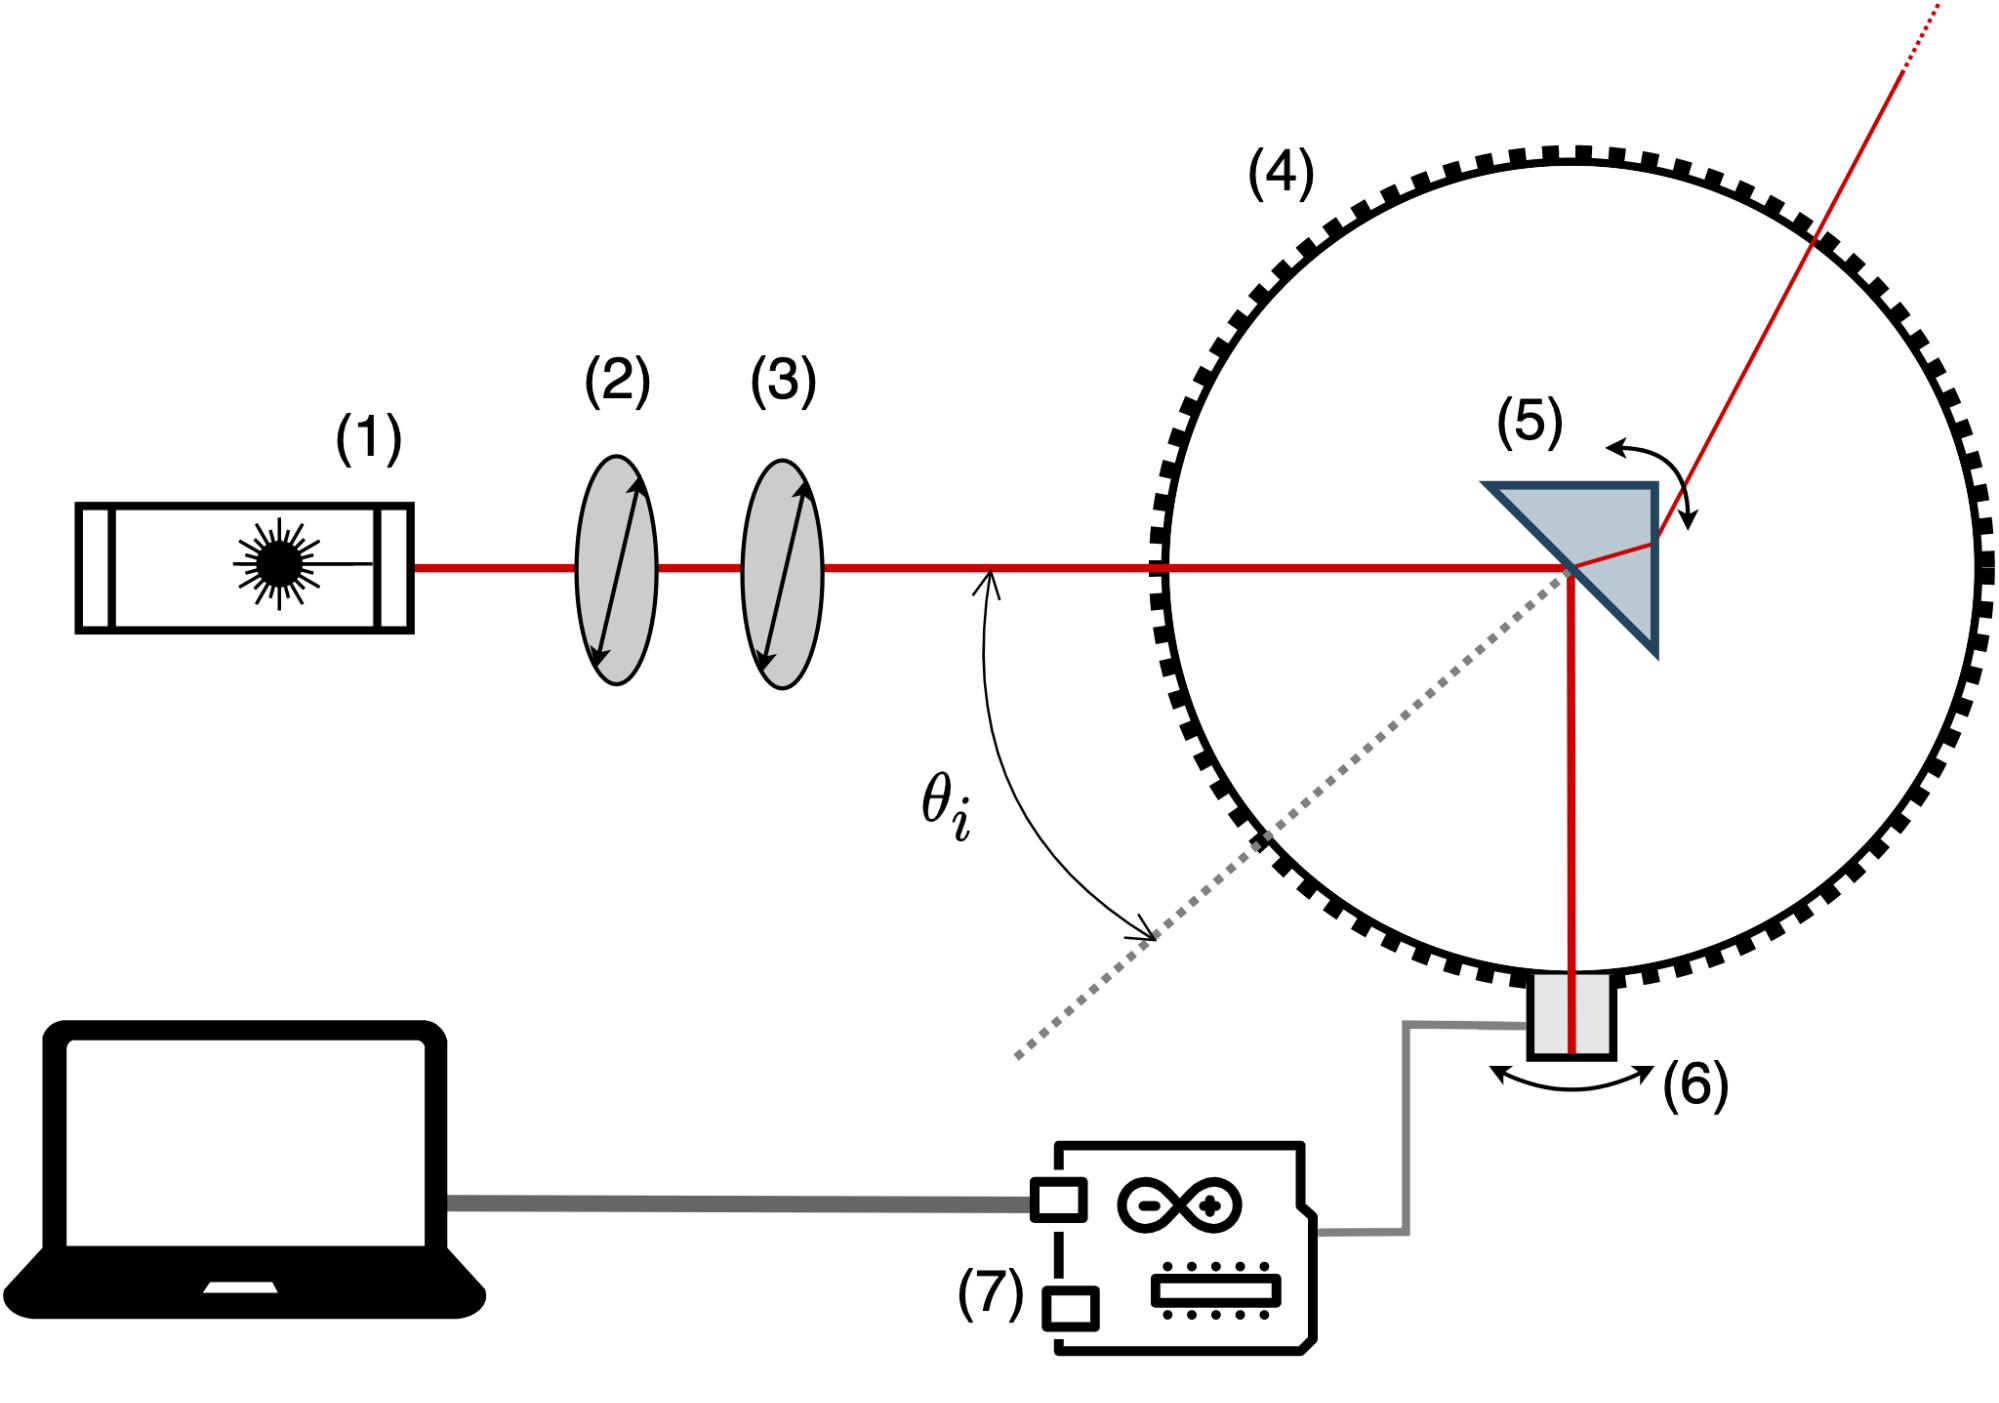
\includegraphics[width=7cm]{instrumental-apparatus.png}
      \caption{
        \emph{
          Apparato sperimentale. A partire da sinistra, in senso orario,
          si trovano: laser(1), filtri polaroid(2, 3), guida circolare(4),
          prisma(5), sensore(6), Arduino(7). Il servomotore non è riportato.
        }
      }
      \label{fig:apparato-strumentale}
    \end{subfigure}%
    \hspace{20mm}
    \begin{subfigure}{.4\textwidth}
      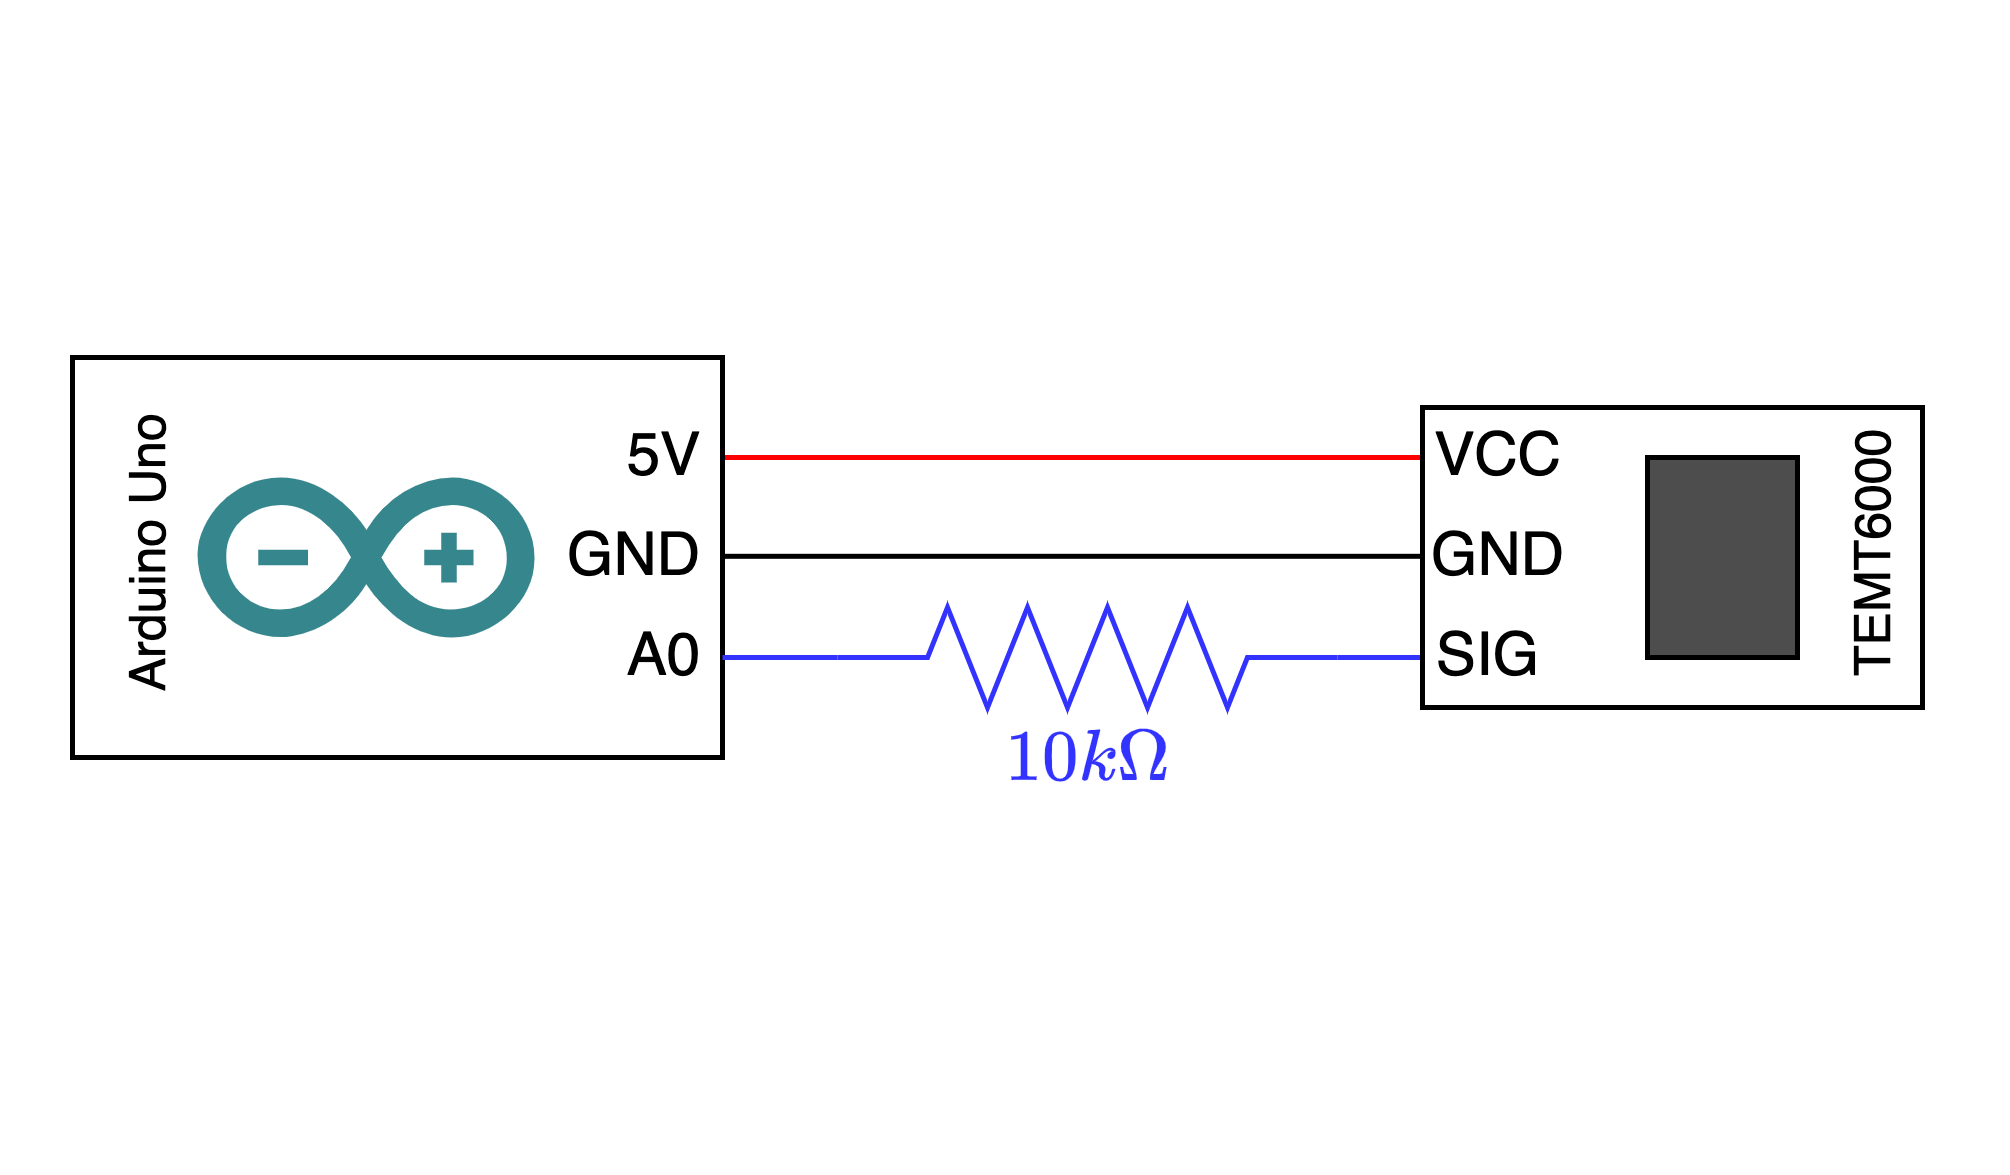
\includegraphics[width=7cm]{circuit-diagram.png}
      \caption{
        \emph{
          Schema circuitale. I pin $\text{VCC}$ e $\text{GND}$ del sensore sono collegati
          all'alimentazione di Arduino. Il pin $\text{SIG}$
          del sensore è collegato ad un input analogico di Arduino, tramite una
          resistenza da $10k\Omega$.
        }
      }
      \label{fig:diagramma-circuito}
    \end{subfigure}
  \end{figure}
%
\subsection{Procedura sperimentale}\label{subsec:procedura-sperimentale}
  Abbiamo seguito la procedura sperimentale riportata di seguito, ripetuta due
  volte (così come indicato nel punto 5): una per raccogliere i dati relativi a $R_\pi$ e una per i dati relativi
  a $R_\sigma$. Questo procedimento è stato adattato da quanto descritto in Lipson\cite{lipson20}.
  \begin{enumerate}
    \item%
      Abbiamo iniziato posizionando il polaroid(3) in modo che la polarizzazione del
      fascio laser fosse parallela al lato del prisma, e abbiamo aggiustato l'angolo
      del laser rispetto al polaroid(3), in modo da evitare che il fascio
      polarizzato uscente dal laser venisse bloccato dal polaroid(3).
    \item%
      Abbiamo posizionato il sensore e il prisma in modo da rendere
      massimo l'angolo $\theta_i$, con il vincolo che
      tutto il fascio laser fosse contenuto sulla superficie del prisma(5)\footnote{Per $\theta_i \to 90^\circ$, la
      proiezione del fascio laser sul prisma è un ellisse di semiasse maggiore $a \to +\infty$. Chiaramente, non appena
      $a$ supera la lunghezza del lato del prisma, le equazioni \eqref{eq:fresnel-eq-p} e \eqref{eq:fresnel-eq-s} perdono
      la loro validità.}
    \item%
      Ruotando il polaroid(2), abbiamo ridotto l’intensità del fascio laser
      incidente al prisma, fino a che Arduino non ha potuto rilevare una
      variazione significativa del segnale del sensore.
      Questo ci ha permesso di sfruttare l'intero range di operatività di Arduino.
    \item%
      Abbiamo raccolto l'intensità luminosa letta dal sensore in questo punto,
      poi abbiamo ruotato il prisma in senso orario e abbiamo
      allineato il sensore di conseguenza.
    \item%
      Abbiamo ripetuto il passo precedente fino a raggiungere un valore di $\theta_i$
      il più possibile vicino a zero
    \item%
      abbiamo ruotato di $90^\circ$ il polaroid(3) e ripetuto l'intera
      procedura un'altra volta.
  \end{enumerate}
%
  I dati che abbiamo raccolto in questo modo non \emph{non} sono
  i coefficienti $R_\pi$ e $R_\sigma$, ma differiscono da essi per una costante
  moltiplicativa, che verrà determinata tramite un \emph{fit}\footnote{Avremmo potuto misurare
  questo valore direttamente, ma in questo caso avremmo dovuto
  abbassare ulteriormente l'intensità del fascio laser, diminuendo la precisione dei
  dati raccolti.}, come descritto in Sez.$\ref{subsec:analisi-dati}$.
\endinput

